\documentclass[aspectratio=169]{beamer}

\usepackage[utf8]{inputenc}
\usepackage{minted,tcolorbox,ulem,listings}
\usepackage{hyperref}

\title{Onion Architecture}
\author{Ethan Kent}
\institute{Spoonflower}
\date{\today}

\begin{document}

\frame{\titlepage}

\begin{frame}
  \frametitle{AKA—}
  \begin{itemize}
    \item Hexagonal Architecture
    \item Ports and Adapters
    \item Clean Architecture
  \end{itemize}

  \vspace{1em}

  Why? People have books to sell and blog posts to write, more or less?
\end{frame}

\begin{frame}
  \frametitle{Dependency Inversion Principle}
  Per Wikipedia:

  \begin{enumerate}
    \item High-level modules should not import anything from low-level modules. Both should depend on abstractions (e.g., interfaces).
    \item Abstractions should not depend on details. Details (concrete implementations) should depend on abstractions.
  \end{enumerate}

\end{frame}

\begin{frame}
  \frametitle{Dependency Inversion Principle, continued}

  \begin{itemize}
    \item Don't refer to volatile concrete classes. Refer to abstract
          interfaces instead.  This rule applies in all languages, whether
          statically or dynamically typed.~.~.~.
    \item Don't derive from volatile concrete classes. This is a corollary to
          the previous rule, but it bears special mention.~.~.~.
    \item Never mention the name of anything concrete and volatile. This is
          really just a restatement of the principle itself.
  \end{itemize}
  \vspace{1em}

  Robert C. Martin, \textit{Clean Architecture} 89 (2018).
\end{frame}

\begin{frame}
  \frametitle{Dependency Inversion Principle, continued}

  This is all pretty abstract. What are you actually saying?
\end{frame}

\begin{frame}
  \frametitle{Dependency Inversion Principle, continued}

  Let's say I have two concepts:

  \begin{itemize}
    \item A \textsc{User}, and
    \item an Express server with a \texttt{POST} endpoint called
          \texttt{updateUser}, which takes in a \textsc{json} payload and
          updates the PostgreSQL database to match the payload, and which server
          emits traces and metrics via Open Telemetry, and also checks a JWT
          bearer token to ensure the \texttt{admin} role is set properly.
  \end{itemize}

  \vspace{1em}

  Which is more stable, less likely to change, closest to our business domain,
  etc.?
\end{frame}

\begin{frame}[fragile]
  \frametitle{Dependency Inversion Principle, continued}
  Should our \texttt{User} type include this data?
  \vspace{1em}
  \begin{minted}{typescript}
interface User {
  givenName: string;
  middleName?: string;
  familyName: string;
  sqlId: number;
  roleFromToken: string;
  oTelCorrelationId: string;
  isAuthorizedToUpdate: boolean;
}
  \end{minted}
\end{frame}


\begin{frame}
  \frametitle{Dependency Inversion Principle, continued}
  \begin{quote}
    High-level modules should not import anything from low-level modules. Both
    should depend on abstractions (e.g., interfaces).
    \vspace{1em}
    \\
    Abstractions should not depend on details. Details (concrete
    implementations) should depend on abstractions.
  \end{quote}
\end{frame}

\begin{frame}
  \frametitle{Dependency Inversion Principle, continued}
  Why?
  \vspace{1em}
  \\
  \begin{quote}
    Depend in the direction of stability. \\

    Designs cannot be completely static. Some volatility is necessary if the
    design is to be maintained.~.~.~. Some~.~.~. components are designed to be
    volatile.  We expect them to change. \\

    Any component that we expect to be volatile should not be depended on by a
    component that is difficult to change.  Otherwise, the volatile component
    will also be difficult to change.
  \end{quote}\\
  \vspace{1em}
  Martin, \textit{supra}, at 120.
\end{frame}

\begin{frame}
  \frametitle{Dependency Inversion Principle, continued}
  Let's apply this thinking to our \texttt{User} type.

  \begin{itemize}
    \item Are \texttt{User}s supposed to be volatile?
    \item Will \texttt{User}s stop having names?
    \item Will our application always use SQL?
    \item Would a business stakeholder recognize an Open Telemetry correlation
          ID as part of the concept of a \textsc{User} in the ubiquitous
          language of the business domain?
  \end{itemize}
\end{frame}

\begin{frame}
  \frametitle{Dependency Inversion Principle, continued}
  In what way are we violating the Dependency Inversion Principle?
  \begin{itemize}
    \item A \texttt{User} is not supposed to be volatile, so it is the kind of
          thing that belongs in a low-level module.
    \item SQL, Open Telemetry, Express, Bearer Tokens, etc., are volatile,
          and so belong in high-level modules.
    \item Our \texttt{User}, in a low-level module, depends here on numerous
          high-level modules.
  \end{itemize}
\end{frame}

\begin{frame}
  \frametitle{Dependency Inversion Principle, continued}
  Okay, this makes sense, but this whole ``rely on abstraction not concretions''
  thing is a bunch of mumbo-jumbo.
\end{frame}

\begin{frame}
  \frametitle{Dependency Inversion Principle, continued}
  Fair enough.

  \vspace{1em}

  Sometimes it will be necessary for lower-level modules to interact.

  \vspace{1em}

  For example, it may be stable, non-volatile, fundamental to the business
  domain, etc.\ that---

  \begin{itemize}
    \item A \textsc{User} is authorized to do some things but not
          others.
    \item A \textsc{User} will be stored somewhere.
    \item The performance of the system will be monitored.
  \end{itemize}
\end{frame}

\begin{frame}[fragile]
  \frametitle{Dependency Inversion Principle, continued}
  We're going to be very careful to have a \texttt{User} type that is abstract
  and non-volatile, more or less in the very deepest, most core part of the
  application:

  \vspace{1em}

  \begin{minted}{typescript}
interface User {
  givenName: string;
  middleName?: string;
  familyName: string;
}
  \end{minted}

  \vspace{1em}

  Sure the \textsc{User} concept will be depended on by other, less general
  things, but the opposite shouldn't happen.
\end{frame}

\begin{frame}[fragile]
  \frametitle{Dependency Inversion Principle, continued}
  But now we have a conflict:

  \begin{itemize}
    \item The \emph{idea} of \textsc{Logging} is pretty abstract, but the
          \emph{implementation} via, say, \textsc{Pino} or \textsc{Winston} is
          concrete.
    \item The \emph{idea} of \textsc{Authorization} is pretty abstract, but the
          \emph{implementation} via, say, an \textsc{OAuth2}-compatible Bearer
          Token is concrete.
    \item \emph{Within} our \emph{abstract} notion of \textsc{Authorization}, we
          may want to refer to the \emph{abstract} notion of \textsc{Logging}, or
    \item Within our \emph{concrete} implementation of \textsc{Authorization} via an
          \textsc{OAuth2}-compatible Bearer Token, we might want to refer to the
          \emph{abstract} notion of \textsc{Logging} in order to avoid unnecessary
          coupling between different concerns.
  \end{itemize}
\end{frame}

\begin{frame}
  \frametitle{Dependency Inversion Principle, continued}
  In short, we sometimes want something more abstract and stable to have the
  notion of some other concept that is more volatile. Perhaps our abstract
  concept of a \textsc{Logger} needs to depend on the details of
  an \textsc{ID} that comes from the \emph{concrete} implementation of the
  abstract idea of \textsc{Persistence}.
\end{frame}

\begin{frame}
  \frametitle{Dependency Inversion Principle, continued}
  Let's pause for a second. Are you starting to get a mental image of layers
  here? And develop an instinct about which way things inside those layers
  should or should not know about one another?
\end{frame}

\begin{frame}
  \frametitle{Dependency Inversion Principle, continued}
  Back to the Dependency-Inversion Principle. How can a more abstract thing talk
  to a more concrete thing?

  \vspace{1em}

  \begin{quote}
    Abstractions should not depend on details. Details (concrete implementations) should depend on abstractions.
  \end{quote}
\end{frame}


\begin{frame}[fragile]
  \frametitle{Dependency Inversion Principle, continued}
  Define an abstraction:

  \vspace{1em}

  \begin{minted}[fontsize=\footnotesize]{typescript}
import { User } from "../core/user";

/** Represents the ability to persist user data asynchronously. */
export interface PersistenceService<Id> {
  /** Get a user by ID. */
  getUser: (id: Id) => Promise<User | null>;
  /** Get all users. */
  getUsers: () => Promise<User[]>;
  /** Update a user, returning the ID on success. */
  insertUser: (user: User) => Promise<Id>;
}
\end{minted}
\end{frame}

\begin{frame}[fragile]
  \frametitle{Dependency Inversion Principle, continued}
  Define some concretions (the details aren't important---what's important is
  that they \emph{are} details):

  \vspace{1em}

  \begin{minted}[fontsize=\tiny]{typescript}
import { Client } from "pg";
import { User } from "../core/user";
import { PersistenceService } from "../services/persistence-service";

const pgClient = new Client();

export const postgresPersistenceProvider: PersistenceService<number> = {
  getUser: async (id: number): Promise<User | null> => {
    pgClient.connect();

    const res = await pgClient.query("SELECT * FROM users WHERE id = $1", [id]);
    await pgClient.end();

    if (res.rowCount === 0) return null;
    if (res.rowCount > 1) throw new Error("Multiple users with the same ID");

    const { givenName, middleName, familyName } = res.rows[0];

    if (!givenName || !familyName) throw new Error("Invalid user");

    return { givenName, middleName, familyName };
  }, // ...
  \end{minted}
\end{frame}

\begin{frame}[fragile]
  \frametitle{Dependency Inversion Principle, continued}
  Define some more concretions (the details aren't important---what's important
  is that they \emph{are} details):
  \begin{minted}[fontsize=\tiny]{typescript}
  // ...
  getUsers: async (): Promise<User[]> => {
    pgClient.connect();

    const res = await pgClient.query("SELECT * FROM users");
    await pgClient.end();

    return res.rows.map((row) => {
      const { givenName, middleName, familyName } = row;

      if (!givenName || !familyName) throw new Error("Invalid user");

      return { givenName, middleName, familyName };
    });
  },

  insertUser: async (user: User): Promise<number> => {
    pgClient.connect();

    const { givenName, middleName, familyName } = user;
    const id = await pgClient.query(
      "INSERT INTO users (given_name, middle_name, family_name) VALUES ($1, $2, $3) RETURNING id",
      [givenName, middleName, familyName]
    );

    await pgClient.end();
    return id.rows[0].id;
  },
};
  \end{minted}
\end{frame}

\begin{frame}[fragile]
  \frametitle{Dependency Inversion Principle, continued}
  Define a different concretion (the details aren't important---what's important
  is that they \emph{are} details):

  \vspace{1em}

  \begin{minted}[fontsize=\scriptsize]{typescript}
import { User } from "../core/user";
import { PersistenceService } from "../services/persistence-service";
import { v4 } from "uuid";

const memoryDb = new Map<string, User>();

export const inMemoryPersistenceProvider: PersistenceService<string> = {
  getUser: (id: string): Promise<User | null> =>
    Promise.resolve(memoryDb.get(id) ?? null),

  getUsers: () => Promise.resolve([...memoryDb.values()]),

  insertUser: (user: User): Promise<string> => {
    const id = v4();
    memoryDb.set(id, user);
    return Promise.resolve(id);
  },
};
  \end{minted}
\end{frame}

\begin{frame}
  \frametitle{Dependency Inversion Principle, continued}
  Okay, so what's the pattern here?

  \begin{itemize}
    \item The \texttt{User} interface is very abstract and depends on nothing
          else.
    \item The service interfaces (\texttt{PersistenceService}) are fairly
          abstract and generic, and are designed to give our application exactly
          the functionality we want.
    \item The service implementations (e.g.
          \texttt{postgresPersistenceProvider}) are very concrete---and kind of
          gross.  They hide away all the tangled wires and allow us to use
          service interfaces that we designed for our application.
  \end{itemize}
\end{frame}

\begin{frame}
  \frametitle{Onion/Clean/Hexagonal Architecture}
  \centering
  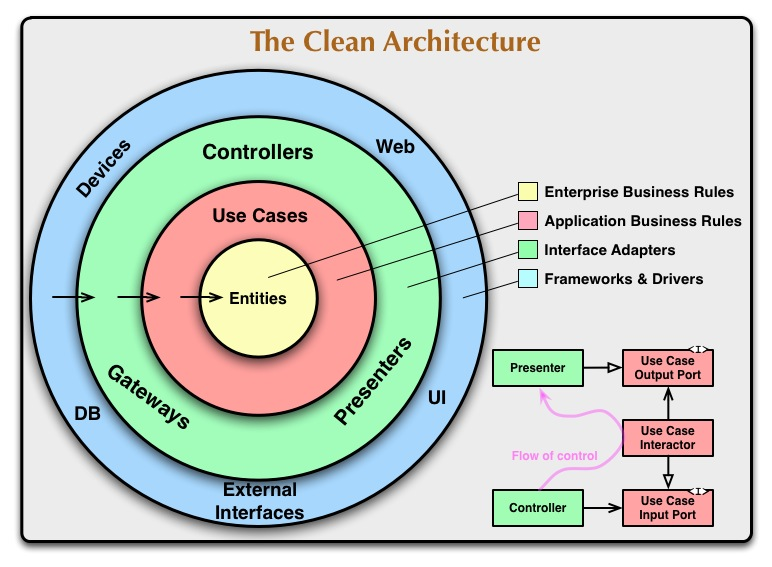
\includegraphics[height=0.8\textheight]{CleanArchitecture.jpg}
\end{frame}

\begin{frame}
  \frametitle{Dependency Inversion Principle, briefly revisited}
  Hang on, is this the same thing as Dependency \textit{Injection}?
\end{frame}

\begin{frame}[fragile]
  \frametitle{Dependency Inversion Principle, briefly revisited}
  They are both use abstractions to ``invert control.'' Specifically, they both
  involve using an abstract way of referring to a component's dependencies.

  \begin{itemize}
    \item Dependency Inversion is a broad design principle saying that we should
          wire things up so that stable things aren't directly aware of more
          volatile things, referring to them more abstractly (``a mid-day flight
          from London'' rather than ``American 173'').
    \item Dependency Injection is a specific technique of passing dependencies
          to components rather than having the components directly contain those
          dependencies.
  \end{itemize}

  \vspace{1em}

  \begin{minted}[fontsize=\scriptsize]{typescript}
const printTimeDI = (timeGetter: () => Date) =>
  console.log(timeGetter().toISOString());

// In prod
printTimeDI(() => new Date());
// In tests
printTimeDI(() => new Date("2022-07-29T21:23:16.438Z"))

  \end{minted}
\end{frame}

\begin{frame}
  \frametitle{And now, to some code}
  $\cdots$
\end{frame}
\end{document}
